%\section{Experimental Methodology}
\section{Experiments}
\label{sec:experimentalmethodology}

In this section, we discuss our method for evaluating the performance of the proposed memory system. We utilize the PARSEC v2.1 and v3.0 benchmark suites with the gem5 simulator~\cite{bienia09parsec2, parsec_2_1_m5} to generate memory traces. Next, we run the Ramulator DRAM simulator to measure the performance of the proposed memory system. Next, we compare the baseline performance of the Ramulator DRAM simulator~\cite{Ramulator} against a modified version which implements the proposed system.

\subsection{Memory Trace Generation}
The PARSEC benchmark suite was developed for chip multiprocessors and is composed of a diverse set of multithreaded applications~\cite{bienia09parsec2}. These benchmarks allow us to observe how the proposed memory system performs in dense memory access scenarios. 
%A number of input sets are provided alongside the PARSEC benchmarks. To run the PARSEC applications, we use the gem5 simulator~\cite{parsec_2_1_m5}.
%
The gem5 simulator~\cite{parsec_2_1_m5} allows us to select the processor configuration used when generating the memory traces. We use $8$ processors in all simulations. The PARSEC traces can be split into regions based on computation type. We focus on regions which feature parallel processing they have the greatest likelihood of bank conflicts.
%
%\subsection{PARSEC Trace Attributes}

Many attributes affect the performance of our proposed memory system, most importantly the density of traces, the overlap of memory accesses among processors, and the stationarity of heavily utilized memory regions. Appendix~\ref{sec:parsec_motivation} shows example PARSEC traces with favorable attributes, \textit{i.e.} they are likely to result in many preventable bank conflicts.

We augment the PARSEC benchmarks in two ways to test our system in additional scenarios, shown in Figures~\ref{fig:vips_split} and~\ref{fig:vips_ramp}, respectively. First we split the given memory bands to simulate an increased number of bands in the system. Next, we introduce dynamic memory access patterns by adding a linear ramp to the previously static address locations. 

\begin{figure}[htbp]
		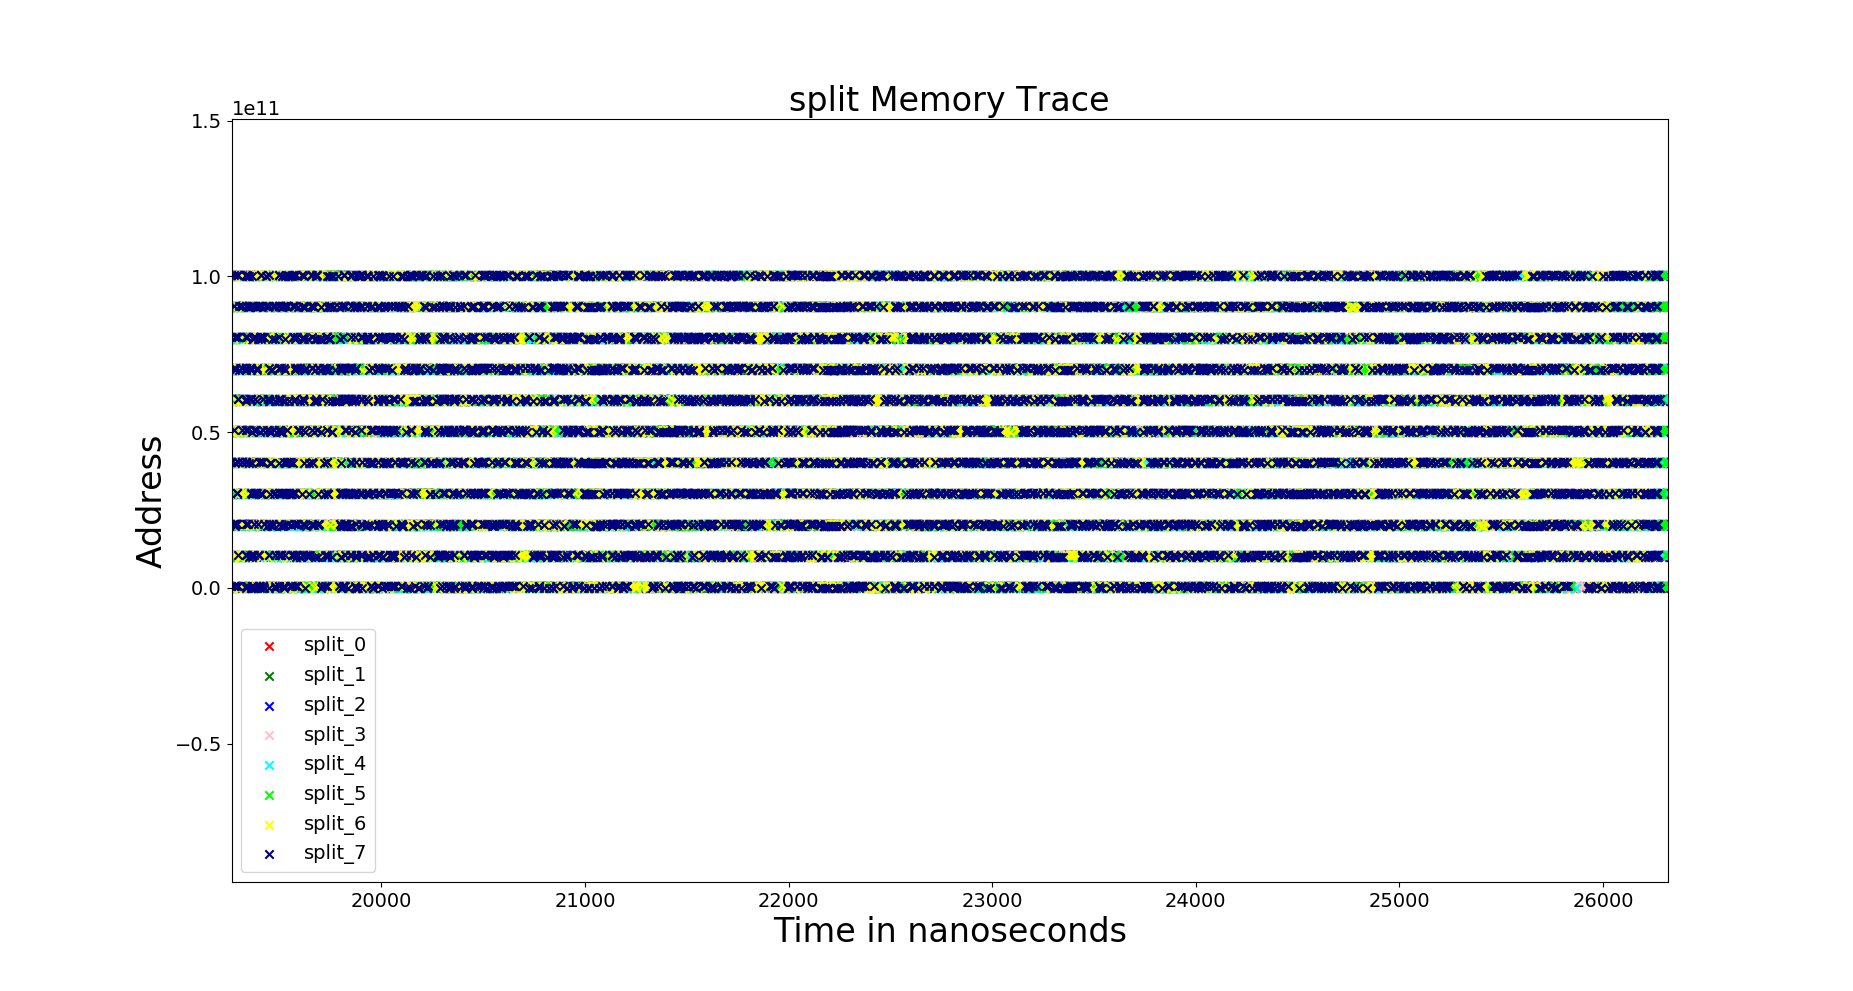
\includegraphics[width=\linewidth]{fig/vips_split.png}
		\caption{\it{The vips benchmark after splitting the primary access bands into multiple additional bands.}}
		\label{fig:vips_split}
\end{figure}


\begin{figure}[htbp]
		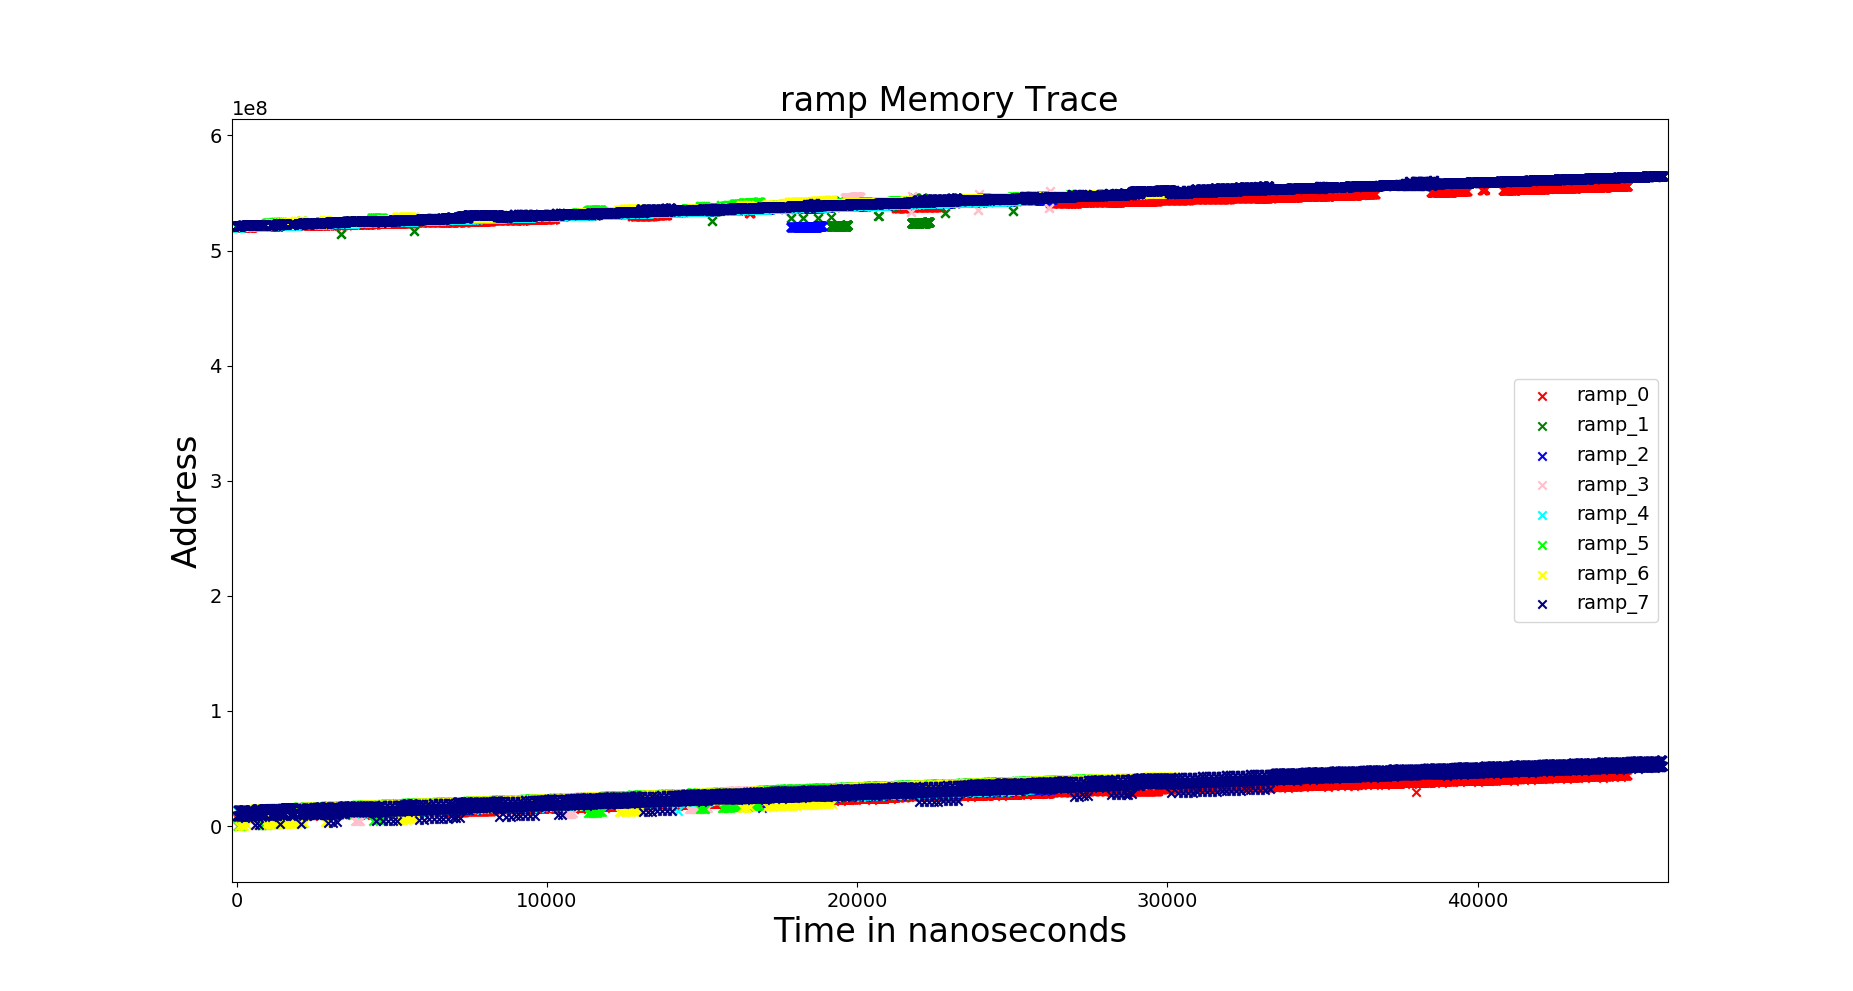
\includegraphics[width=\linewidth]{fig/vips_ramp.png}
		\caption{\it{The vips benchmark after adding a ramp to the major memory bands.}}
		\label{fig:vips_ramp}
\end{figure}


\subsection{Ramulator}

We use the Ramulator DRAM simulator to compare the number of CPU cycles required to execute the PARSEC memory traces. First, we use the original Ramulator simulator to measure a baseline number of CPU cycles. Then we implement the proposed memory system and use the modified Ramulator (fixing all other configuration) to calculate improvements over the baseline. Our simulations vary the overhead parameter $\alpha$.

%
%the memory system is permitted to use. 
%The following are the specifics of the Ramulator configuration file used to acquire the simulation results:
%\begin{itemize}
%\item Standard : HBM
%\item Channels: 8
%\item Ranks: 1
%\item Speed: 1 Gigabits per second
%\item Organization: 4 Gigabits
%\item CPU ticks: 32
%\item Memory ticks: 5
%\end{itemize}
%}